% Schematic: preference forming across depth (companion to a real data plot).
% Two reward-lens traces start tangled and flat near zero, stay tangled through
% the middle layers, then split hard in the last ~20%: chosen rises, rejected
% falls. A dashed line marks the crystallization depth (~90%).
% Compile with ../build_figures.sh -> content/assets/figures/accumulation.svg
\documentclass[border=10pt]{standalone}
\usepackage{tikz}
\usetikzlibrary{calc,arrows.meta}
\definecolor{rlink}{HTML}{3F51B5}    % chosen
\definecolor{raccent}{HTML}{FF5722}  % crystallization / margin
\definecolor{rmuted}{HTML}{6B7280}   % rejected / axes
\begin{document}
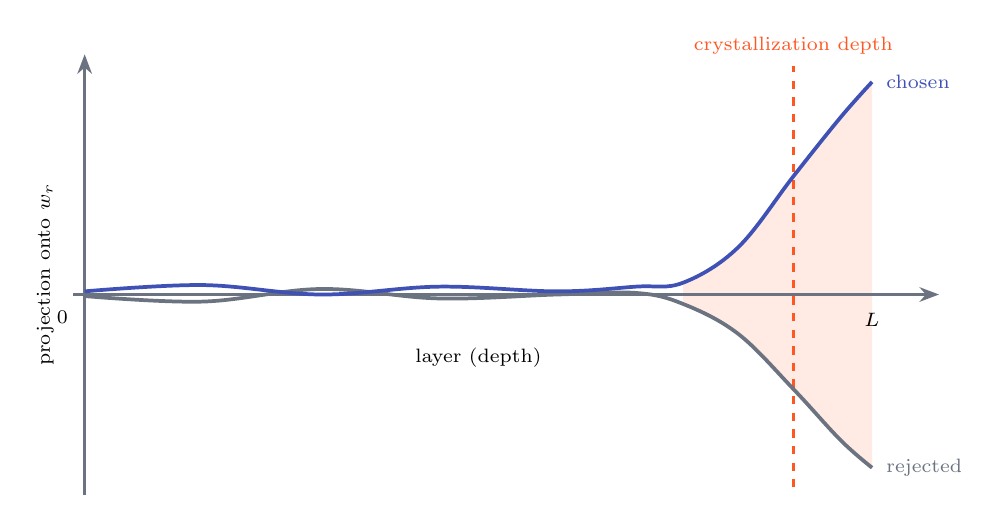
\begin{tikzpicture}[>=Stealth, line width=0.9pt, font=\small]
  % x: layer 0..10 (= L), drawn in cm.  y: projection onto w_r, ~ -2.5..3.

  % growing-margin shading (under the curves)
  \fill[raccent!12]
     plot[smooth,tension=0.6] coordinates
       {(7.6,0.15) (8.3,0.6) (9,1.5) (9.6,2.25) (10,2.7)}
     -- plot[smooth,tension=0.6] coordinates
       {(10,-2.2) (9.6,-1.85) (9,-1.2) (8.3,-0.5) (7.6,-0.12)}
     -- cycle;

  % crystallization depth (drawn under the curves)
  \draw[raccent, dashed, line width=1.0pt] (9,-2.45) -- (9,2.9);
  \node[raccent, font=\scriptsize, anchor=south] at (9,2.92) {crystallization depth};

  % axes
  \draw[rmuted, ->, line width=0.9pt] (-0.15,0) -- (10.85,0);
  \draw[rmuted, ->, line width=0.9pt] (0,-2.55) -- (0,3.05);
  \node[black, font=\scriptsize, anchor=north east] at (-0.08,-0.08) {$0$};
  \node[black, font=\scriptsize, anchor=north] at (10,-0.1) {$L$};
  \node[black, font=\scriptsize, anchor=north] at (5,-0.55) {layer (depth)};
  \node[black, font=\scriptsize, rotate=90] at (-0.5,0.25) {projection onto $w_r$};

  % rejected trace
  \draw[rmuted, line width=1.35pt]
     plot[smooth,tension=0.6] coordinates
     {(0,-0.02) (1.5,-0.09) (3,0.07) (4.5,-0.05) (6,0.0) (7,0.02)
      (7.6,-0.12) (8.3,-0.5) (9,-1.2) (9.6,-1.85) (10,-2.2)};
  % chosen trace
  \draw[rlink, line width=1.35pt]
     plot[smooth,tension=0.6] coordinates
     {(0,0.04) (1.5,0.12) (3,0.0) (4.5,0.1) (6,0.04) (7,0.1)
      (7.6,0.15) (8.3,0.6) (9,1.5) (9.6,2.25) (10,2.7)};

  % trace labels
  \node[rlink, font=\scriptsize, anchor=west] at (10.05,2.7) {chosen};
  \node[rmuted, font=\scriptsize, anchor=west] at (10.05,-2.2) {rejected};
\end{tikzpicture}
\end{document}
